% This paper by Raychev describes parallelizing user-defined aggregations
% using Symbolic Execution

% http://research.microsoft.com/pubs/256579/143-raychev.pdf

% Describe the ideas in this paper and see if these ideas could be used for
% OpenMP race detection (inability to parallelize = race). If not, why not, or
% in which cases? Could this help your research in any way?

\begin{refsection}
\section{Questions from Ganesh Gopalakrishnan}
\label{sec:member1}

\subsection{Describe the ideas in this paper\dots}
\label{sec:member11}

The authors in~\cite{Raychev:2015:PUA:2815400.2815418} present a system,
called \symp, that allows a user to automatically parallelize and perform
User-defined aggregations (UDAs) queries, in order to optimize and exploit the
parallelism available in large-scale data-processing systems, such as
MapReduce and Hadoop.
%

\begin{wrapfigure}{l}{0.23\textwidth}
  \centering
  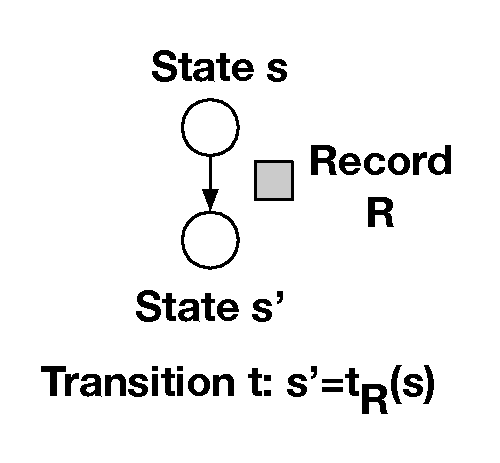
\includegraphics[width=0.23\textwidth]{figures/symple_ex1}
  \caption{Transition on a record $R$ from state $s$ to the next state $s'$.}
  \label{fig:symple_ex1}
\end{wrapfigure}

\noindent
These big systems, in general, provide parallel support for aggregation
functions, such as \emph{Max}, \emph{Count}, \emph{Sum}, since they are easy
to parallelize and allow to obtain high performance.
%
However, complex aggregation queries, such as UDAs, are hard to parallelize
because of their data dependencies (i.e.\ loop-carried data dependency), so
the execution has to be run sequentially introducing a slowdown of several
orders-of-magnitude.
%
For example, if we have a big amount of data (records) that come from the logs
of an e-commerce website and we want to query the \emph{number of reviews per
  user session}, it would be non-trivial to parallelize.
%
\symp provides a mechanism for performing
MapReduce-style~\cite{Dean:2008:MSD:1327452.1327492} aggregate functions,
processing chunks of the divided input in parallel, and running a symbolic
execution of the UDAs where those dependencies are treated as ``unknown''
symbolic values.
%
As a result, the symbolic execution returns a \emph{symbolic summary} which is
basically the output of the UDA as a function of its input.
%
\symp can run in parallel the symbolic executions on each input chunk and
compose the summaries in a final reduction step to produce the result that
would match a sequential execution of the UDA.
\\

\noindent
\paragraph{Symbolic parallelism in detail:}

A given UDA query, that has to be computed by the system, is expressed in a
dialect of C++.
%
The values of variables used by the function for the computation are called
the \emph{State s}.

\begin{wrapfigure}{r}{0.20\textwidth}
  \centering
  \vspace{-15pt}
  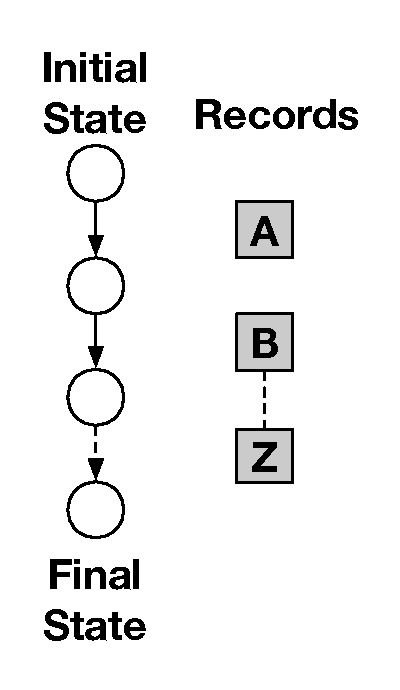
\includegraphics[width=0.18\textwidth]{figures/symple_ex2}
  \vspace{-10pt}
  \caption{Sequential execution of the query on the entire dataset.}
  \label{fig:symple_ex2}
\end{wrapfigure}

\noindent
The operations executed by the query on the records, for example to find the
\emph{number of reviews per user session} (referring to the previous example),
might change the state of the computation, these operations are the
\emph{transitions}.
%
Therefore, a transition for a record \emph{R} changes the current state from
\emph{s} to the next state \emph{s'} as shown in Figure~\ref{fig:symple_ex1}.
%
As stated above, when we have a complex query, it is hard to parallelize
because the next state that the query has to compute always depends on the
previous state, so data dependencies are the real problem.
%
In a sequential execution (Figure~\ref{fig:symple_ex2}), it would not be a
problem since each transition is computed sequentially by only one process.

In order to parallelize such a query using symbolic execution (or
\emph{symbolic parallelism}), \symp proceeds in the following way.
%
Once the input is divided in chunks, the symbolic parallelism mechanism
computes the query \textbf{concretely} on the first chunk, obtaining the state
\textbf{s} as shown in Figure~\ref{fig:symple_ex3}.
%
Now, the symbolic parallelism can execute symbolically, and in parallel the
query on all the other chunks.
%
It means that for each record, in a given chunk, the symbolic execution
applies the transitions starting from a symbolic unknown state \textbf{x}.
%
Figure~\ref{fig:symple_ex4} shows how this computation returns a function
\textbf{F} of $x$, where the transition has been applied on the records $D$,
$E$, and $F$.
%
Finally, we combine the function $F$ on the concrete state $s$ and we obtain
the final state, which would be the result of $F(s) = t_D(t_E(t_F(s)))$.

% \begin{figure}
%   \begin{minipage}[b]{0.3\textwidth}
%     \begin{flushleft}
%       \raisebox{30pt}{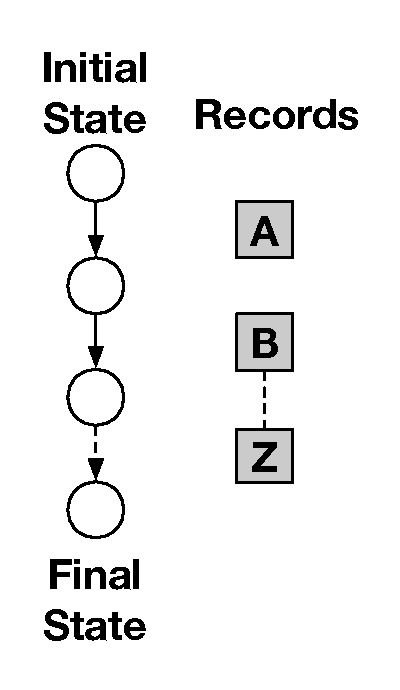
\includegraphics[width=0.6\textwidth]{figures/symple_ex2}}
%       \caption{Sequential execution of the query on the entire dataset.}
%       \label{fig:symple_ex2}
%     \end{flushleft}
%   \end{minipage}
%   \hfill
%   \begin{minipage}[b]{0.3\textwidth}
%     \centering
%     \raisebox{35pt}{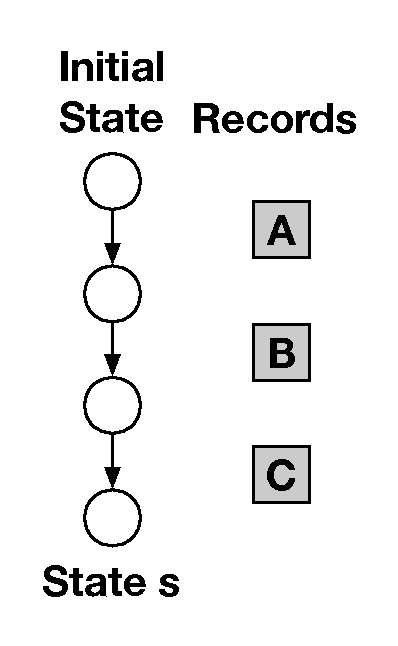
\includegraphics[width=0.65\textwidth]{figures/symple_ex3}}
%     \caption{Concrete execution of the query on the first chunk of data.}
%     \label{fig:symple_ex3}
%   \end{minipage}
%   \hfill
%   \begin{minipage}[b]{0.3\textwidth}
%     \begin{flushright}
%       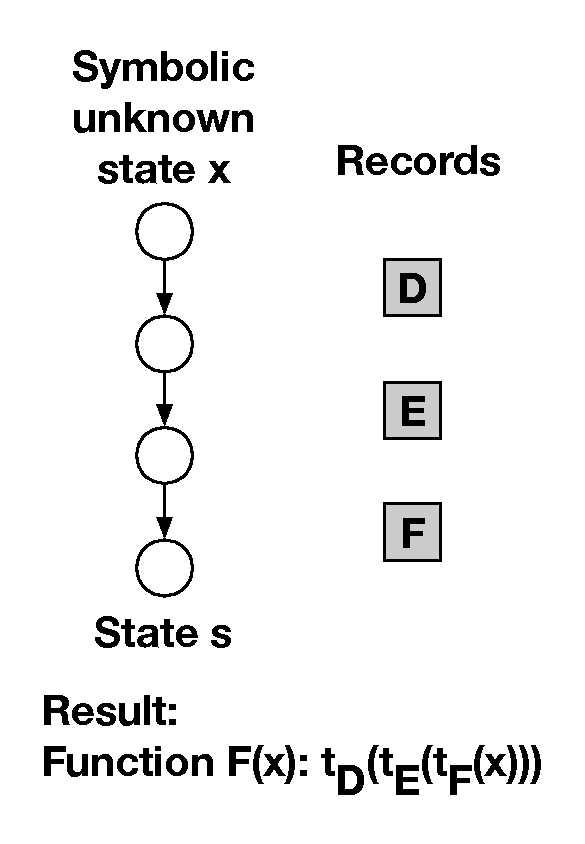
\includegraphics[width=0.8\textwidth]{figures/symple_ex4}
%       \caption{Parallel symbolic execution on the rest of the data chunks.}
%       \label{fig:symple_ex4}
%     \end{flushright}
%   \end{minipage}
% \end{figure}

% \begin{figure}
%   \begin{minipage}[b]{0.3\textwidth}
%     \begin{flushleft}
%       \centering
%       \raisebox{35pt}{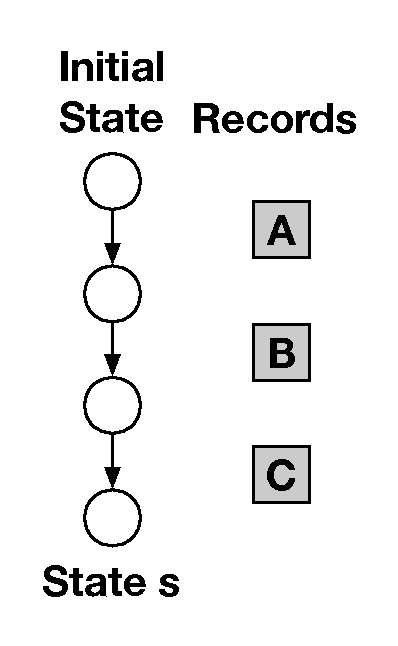
\includegraphics[width=0.65\textwidth]{figures/symple_ex3}}
%       \caption{Concrete execution of the query on the first chunk of data.}
%       \label{fig:symple_ex3}
%     \end{flushleft}
%   \end{minipage}
%   \hfill
%   \begin{minipage}[b]{0.3\textwidth}
%     \centering
%     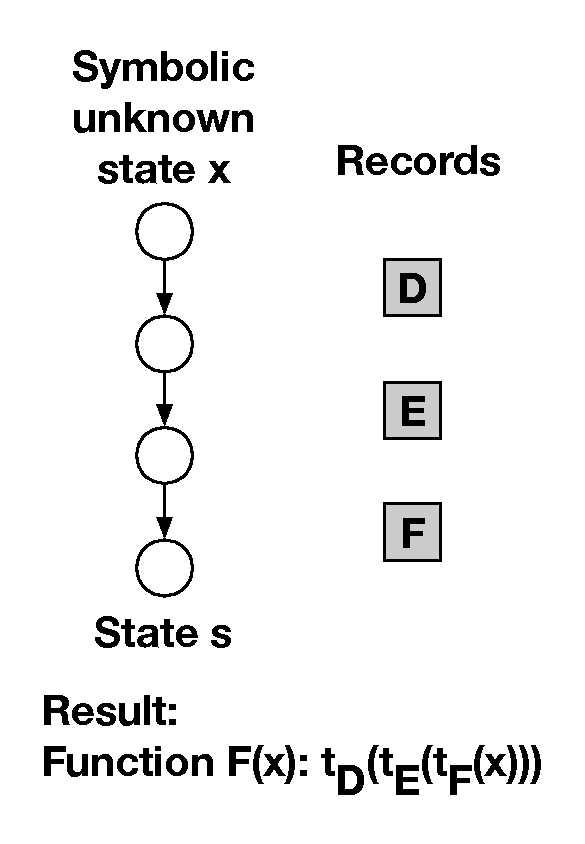
\includegraphics[width=0.8\textwidth]{figures/symple_ex4}
%     \caption{Parallel symbolic execution on the rest of the data chunks.}
%     \label{fig:symple_ex4}
%   \end{minipage}
%   \hfill
%   \begin{minipage}[b]{0.3\textwidth}
%     \begin{flushright}
%       \centering
%       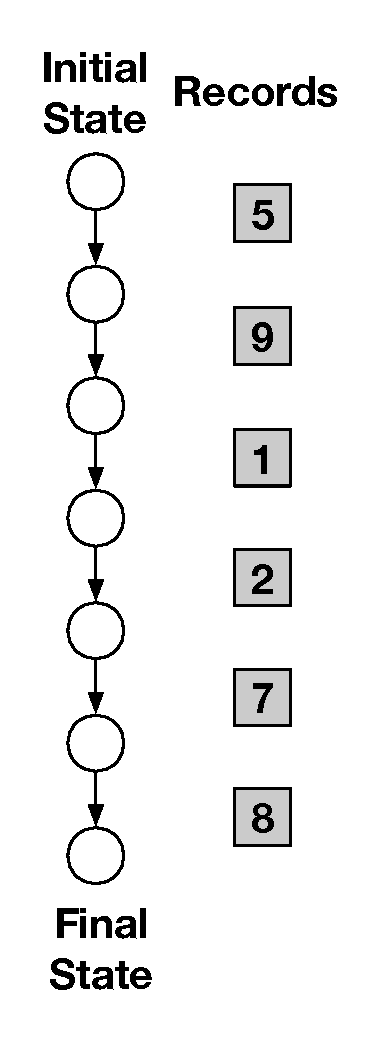
\includegraphics[width=0.6\textwidth]{figures/symple_ex5}
%       \caption{Parallel symbolic execution on the rest of the data chunks.}
%       \label{fig:symple_ex5}
%     \end{flushright}
%   \end{minipage}
% \end{figure}

\begin{figure}
  \begin{minipage}[b]{0.3\textwidth}
    \begin{flushleft}
      \centering
      \raisebox{0pt}{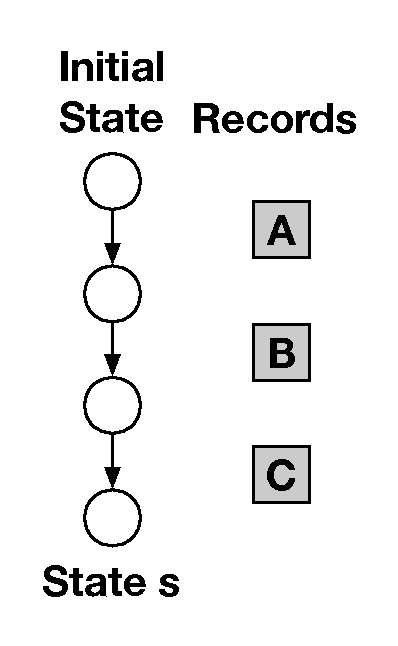
\includegraphics[width=0.6\textwidth]{figures/symple_ex3}}
      \caption{Concrete execution of the query on the first chunk of data.}
      \label{fig:symple_ex3}
    \end{flushleft}
  \end{minipage}
  \hfill
  \begin{minipage}[b]{0.3\textwidth}
    \centering
    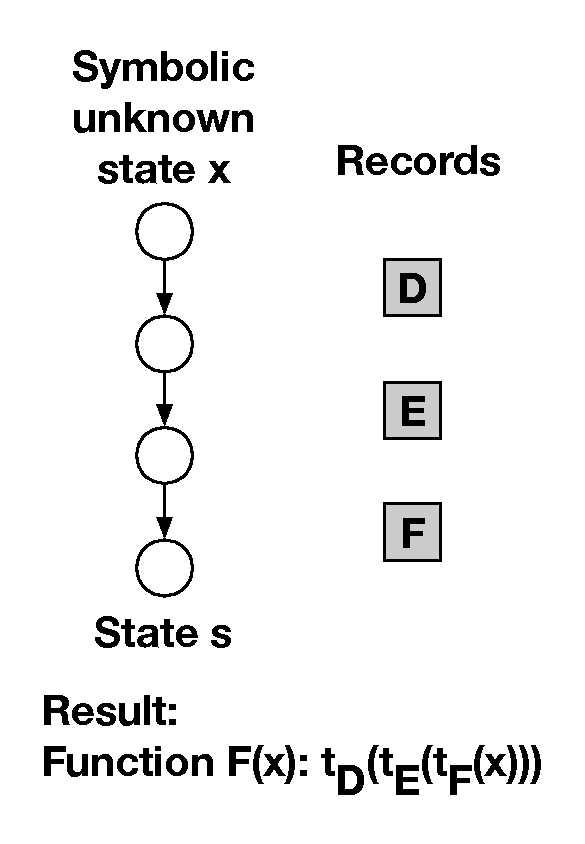
\includegraphics[width=0.8\textwidth]{figures/symple_ex4}
    \caption{Parallel symbolic execution on the rest of the data chunks.}
    \label{fig:symple_ex4}
  \end{minipage}
  \hfill
  \begin{minipage}[b]{0.3\textwidth}
    \begin{flushright}
      \centering
      \raisebox{0pt}{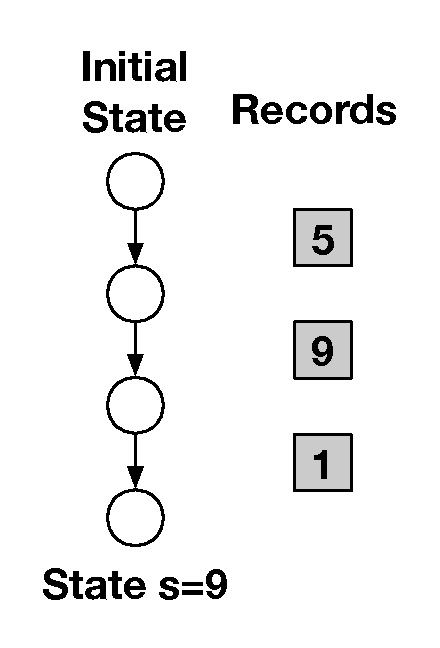
\includegraphics[width=0.6\textwidth]{figures/symple_ex6}}
      \caption{Concrete execution of the query on the first chunk of data.}
      \label{fig:symple_ex6}
    \end{flushright}
  \end{minipage}
\end{figure}

\paragraph*{Example:}
Let us now apply the symbolic parallelism on a real example.
%
Suppose we want to compute the aggregation function $Max$ defined as:

\begin{center}
  \begin{lstlisting}
    if |\textbf{state}| < |\textbf{{\color{blue}value}}| then |\textbf{state}| = |{\textbf{\color{blue}value}}|
  \end{lstlisting}
\end{center}

\noindent
on a list of integers such as $\{5, 9, 1, 2, 7, 8\}$, and divide the integers
into two chunks: $\{5, 9, 1\}$ and $\{2, 7, 8\}$.
%
The computation on the first chunk will execute concretely, so the max value
will be $9$ (Figure~\ref{fig:symple_ex6}).
%
In the meantime, in parallel, the symbolic execution performs the computation
on the second chunk starting from an unknown symbolic state $x$.
%
As shown in Figure~\ref{fig:symple_ex7}, the symbolic execution is executed on
each value of the second chunk and it returns $F$ as a function of $x$.
%
Now, the function $F$ can be combined with the concrete value computed on the
first chunk and the final state will be $F(9)=9$.

Figure~\ref{fig:symple_ex8} shows a complete symbolic pipeline of the same
aggregation function \emph{Max} on the input $\{1, 8, 3, 4, 7, 6, 9, 5, 2\}$.
%
The first step is to split the data in chunks and assign each one of them to a
different task.
%
The second step runs the symbolic executions in parallel (notice that the
first task is always computed concretely).
%
$Task 1$ and $Task 2$ return two functions that are going to be combined with
the initial state computed by $Task 0$.
%
Indeed, the max value computed by $Task 0$, which is $8$ will be used in place
of $x$ in the function returned by $Task 1$.
%
Then, the new value obtained by the first combination will be used with the
function returned by $Task 2$, and the max value computed.

%  \begin{figure}
%   \begin{minipage}[b]{0.4\textwidth}
%     \begin{flushleft}
%       \centering
%       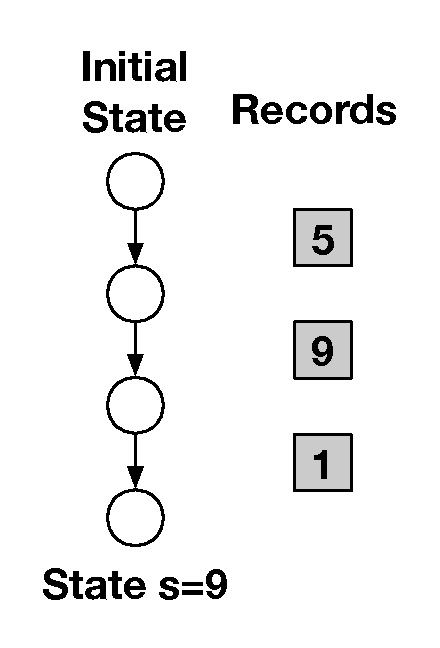
\includegraphics[scale=0.7]{figures/symple_ex6}
%       \caption{Concrete execution of the query on the first chunk of data.}
%       \label{fig:symple_ex6}
%     \end{flushleft}
%   \end{minipage}
%   \hfill
%   \begin{minipage}[b]{0.55\textwidth}
%     \begin{flushright}
%       \centering
%       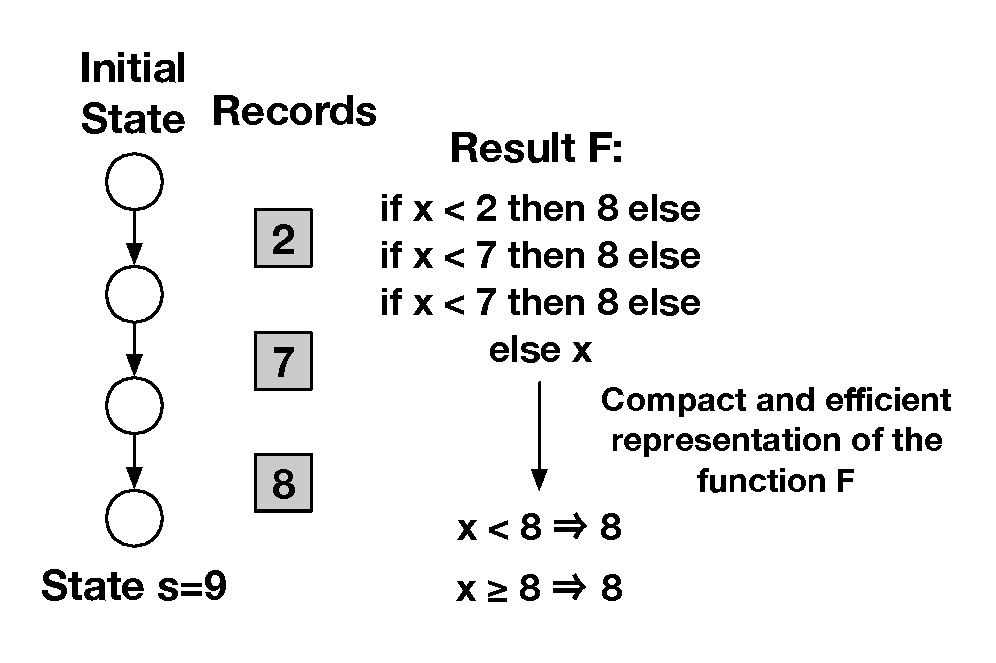
\includegraphics[scale=0.7]{figures/symple_ex7}
%       \caption{Parallel symbolic execution on the rest of the data chunks.}
%       \label{fig:symple_ex7}
%     \end{flushright}
%   \end{minipage}
% \end{figure}

 \begin{figure}[H]
  \begin{minipage}[b]{0.47\textwidth}
    \begin{flushleft}
      \centering
      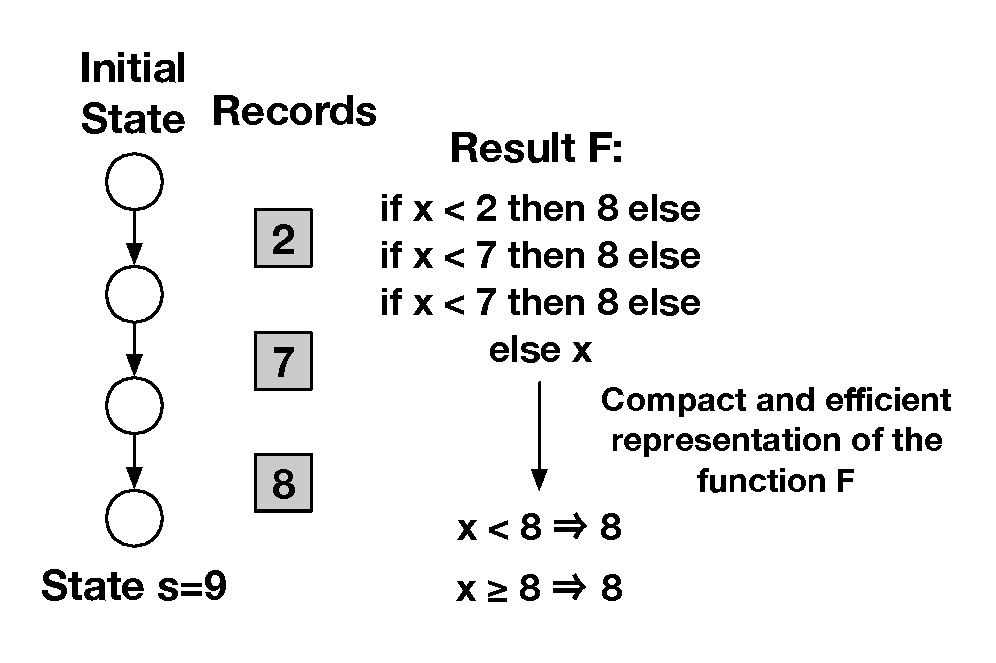
\includegraphics[scale=0.5]{figures/symple_ex7}
      \caption{Parallel symbolic execution on the rest of the data chunks.}
      \label{fig:symple_ex7}
    \end{flushleft}
  \end{minipage}
  \hfill
  \begin{minipage}[b]{0.47\textwidth}
    \begin{flushleft}
      \centering
      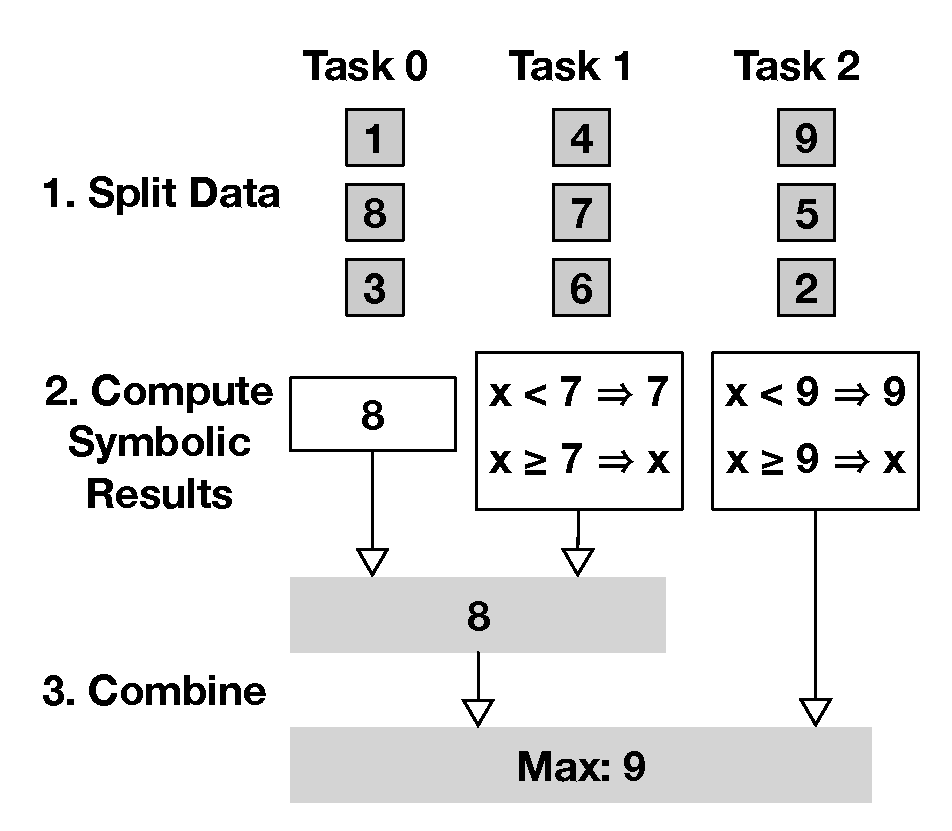
\includegraphics[scale=0.5]{figures/symple_ex8}
      \caption{Full parallel symbolic execution
        pipeline. \textcolor{white}{empty}}
      \label{fig:symple_ex8}
    \end{flushleft}
  \end{minipage}
\end{figure}

% \begin{figure}
%   \centering
%   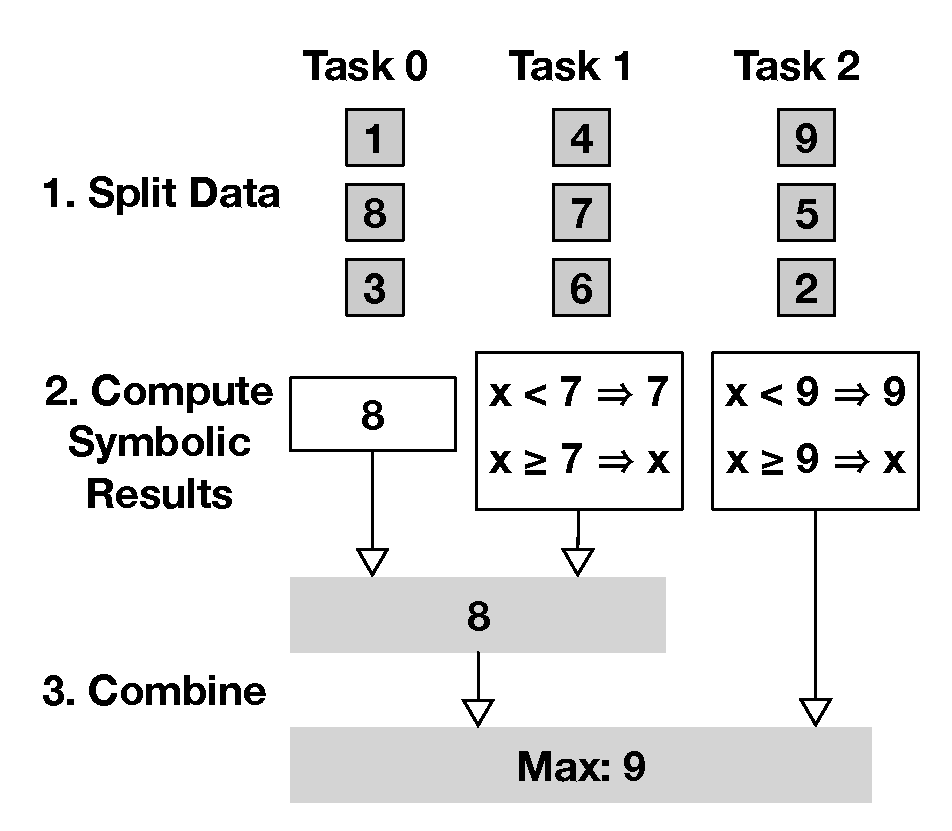
\includegraphics[scale=0.7]{figures/symple_ex8}
%   \caption{Full parallel symbolic execution pipeline.}
%   \label{fig:symple_ex8}
% \end{figure}

\paragraph{Discussion:} In the example of Figure~\ref{fig:symple_ex6} the
symbolic execution computes a function for each value in the data set.
%
This function is actually the result of the symbolic execution as it explores
all the possible paths (i.e.\ of the computation of the query) and accumulates
the path constraints for each decision (as shown in Figure~3
in~\cite{Raychev:2015:PUA:2815400.2815418}).
%
A path constraint implies a function: for instance if the symbolic execution
is computing the aggregation function $Max$ and it is on a state $x$, when it
encounters a value $v$ from the input, it will generate two path constraints
``$x < v \implies max = v$'' and ``$x \geq v \implies max = x$''.
%
The main point in the function generation is its shape, because it influences
the performance of the entire computation.
%
Indeed, \symp introduces its own data types (which look and behave like
standard C++ types) that are the key to control the shape of the functions.

The equivalent of the C++ data type \emph{int} in \symp is called symbolic
integer \emph{SymInt}.
%
The \emph{SymInt} data type has a very specific shape:

\begin{equation*}
x \in [l, u] \implies ax+b
\end{equation*}

This means that if the value of the integer $x$ is in the interval $[l,u]$ the
resulting function is of the form $ax+b$.
%
The \emph{SymInt} data type stores the four constants $l, u, a, b$, that allow
to keep the function always in the shape $ax+b$, and defines transformers to
maintain the function shape.
%
For example:

\begin{itemize}
\item If the state \emph{s} is a concrete value $b$, we have $x \in [l, u] \implies 0x+b$.
\item If the state \emph{s} is a symbolic value $x$, we have $x \in [l, u] \ \implies 1x+0$.
\item If $s = 7$, $x \in [l, u] \implies 0x + 7$.
\item If $(s \leq 5)$, $x \in [l, 5] \implies ax + b$.
\end{itemize}

There are other data types that follow the same idea, such as \emph{SymBool},
\emph{SymEnum}, \emph{SymVector}, and \emph{SymPredicate}. Furthermore \symp
allow the user to define custom data structures through composition of data
types.

\subsection{\dots~and see if these ideas could be used
  for OpenMP race detection (inability to parallelize = race).
  %
  If not, why not, or in which cases?
  %
  Could this help your research in any way?}
\label{sec:member12}

In OpenMP a data race may happen when the programmer parallelizes, with some
of the OpenMP construct, a portion of code (i.e.\ loop) that carries a data
dependency.
%
The compiler does not perform any check on the OpenMP code, therefore if the
developer parallelizes a for-loop like that one in Figure~\ref{fig:race1}, the
compilation result will be a program that might be racy when executed with
multiple threads.
%
\begin{wrapfigure}{R}{0.35\textwidth}
\begin{lstlisting}[language=C]
  #pragma omp parallel for
  for (i = 1; i < N; i++)
     sum = sum + a[i];
\end{lstlisting}
\caption{OpenMP sum parallel reduction loop with a data race on the variable
  $sum$, because of a data dependency and lack of synchronization.}
\label{fig:race1}
\end{wrapfigure}
%
The example in Figure~\ref{fig:race1} performs a reduction of a sum operation,
and has a race condition on the variable $sum$.
%
% Most likely, the example in Figure~\ref{fig:race1}, if executed with two or
% more threads, will manifest a race condition in some of the array locations.
%
Due to the data dependency and the absence of any synchronization mechanism,
two different threads will be allowed to access the location of $sum$
simultaneously, generating the data race.

The system \symp handles the $sum$ reduction by splitting the input for the
function in chunks, and running in parallel the symbolic execution on each
input chunk to compute the intermediate summaries.
%
The results from each symbolic execution will then be combined together to
generate the final result, as seen previously in the description of the
algorithm.
%
The \symp approach does not perform any checks on the aggregation operation,
so basically it does not know if the function has any data dependency or not.
%
The system always performs symbolic execution, even in absence of data
dependency (which would allow it to run in parallel without symbolic
execution).

The authors in the paper do not clarify if the system runs a data dependency
analysis to discover possible data dependencies (and so potential races),
before parallelizing the query.
%
I suspect that, no matter if the function carries some data dependecies or
not, \symp will always run symbolic parallelism.
%
If there are no data dependencies, after a certain number of steps the
symbolic representation will become equivalent to the concrete so it would not
be an issue.
%
On the other hand this approach, in presence of data-dependency-free
functions, introduces some overheads, as there would be a better way to
parallelize.

I believe the symbolic approach of \symp could not be used for my OpenMP data
race detection research.
%
While \symp tries to find an efficient way to parallelize complex UDAs, in
OpenMP programs the code is already parallelized by the programmer, and it
requires some techniques (static or dynamic) to analyze it in order to find
any data races.
%
However, the parallel symbolic executions approach may be useful in improving
existing techniques for data race detection.

The \emph{happens-before} relation is a well-known technique to find,
precisely, data races on threaded programs at runtime~\cite{Flanagan:2009}.
%
On the other hand, it only finds races on branches of the program that are
actually executed, and it also demands many resources, and generates high
runtime and memory overheads.
%
A symbolic execution approach could improve both problems of this dynamic
technique:

\begin{enumerate}
\item \emph{Explore multiple path of the program:} The symbolic execution
  might run the OpenMP program symbolically, generating symbolic memory
  locations (that a thread would access at runtime), executing the program
  operations, and when present the synchronization operations.
  %
  Therefore, the input for a \emph{symbolic happens-before} would be:

  \begin{itemize}
  \item Threads info (i.e. TID)
  \item The ``symbolic addresses'' (per thread).
  \item Per-thread and per-lock vector clocks and/or epochs; updated during
    the symbolic execution of the synchronization operations.
  \item The type of the operations executed (i.e.\ read or write).
  \end{itemize}

  If the relation is not satisfied, which means:
  %
  \begin{blockquote}
    \emph{a symbolic memory location exists, it has been accessed
    by two different threads, at least one of the thread operation is a
    write, and an order of the two events can not be established,}
  \end{blockquote}
  %
  a race is detected and reported.

  In the case of branches, the symbolic execution (i.e.\ based on the data
  types) could generate and explore different paths of the OpenMP program
  spotting more racy behaviors.
\item \emph{Reducing runtime and memory overhead:} The parallel programming
  model of OpenMP is very structured, in the sense that during an execution of
  a program, the OpenMP runtime:
  \begin{enumerate}
  \item Spawns a team of threads when it encounters a parallel section.
  \item Executes the work in parallel.
  \item Destroys the threads team when the parallel section terminates.
  \item The program continues the execution sequentially until the following
    parallel section.
  \end{enumerate}
  %
  This would allow to distribute, across multiple processes (i.e.\ in a
  cluster), the symbolic execution of different parallel sections, while the
  single symbolic execution is itself already parallel and distributed across
  multiple cores.
  %
  An approach like this could mitigate the runtime and memory overhead
  generated by the happens-before technique, and the additional overhead which
  may arise from the multiple paths explored by the symbolic execution.
\end{enumerate}

\printbibliography

\end{refsection}

%%% Local Variables:
%%% mode: latex
%%% eval: (flyspell-mode 1)
%%% TeX-master: "root.tex"
%%% End:
